\chapter{Hardware Design and Implementation}


\section{Mechanical Hardware}
%WHAT you are going to present in this chapter/section
%WHY you are presenting it, and
%HOW you are going to present it
The mechancial design that created the physical model is presented here. The physical model allowed the abstract mathematical model to be implemented and experiments to be conducted. It will be presented by discussing the various components required and design decision made to implement a physical model that represents the mathematical model.\\

Figure \ref{fig:mech_model} shows the physical model designed and used for experiments. It emphasises some of the more critical components that were required.\\

It is important that the physical model holds the assumption made during the derivation of the robotic gymnast. These assumptions include planar dynamics of the robotic gymnast and rigid body dynamics. The assumption of planar dynamics comes in affect with the connection between the rotating shaft and the non-actuated pendulum. If the assumption holds there should be no vibration of the pendulum in any other direction than the rotating plane of the pendulums. 

The assumption of rigid body dynamics is easily met due to the forces acting on the pendulums results in negligible strain.

\subsection{Mechanical Components}
The components emphasised in Figure \ref{fig:mech_model} is discussed in the following section and explains their significance of use.\\

The electrical slipring converts the rotating wires that lead to the motor mounted on non-actuated pendulum to stationary wires allowing for free rotation and easy connection to the electrical design.\\

The bearing housing holds the ball-bearings in place ensuring for no unwanted vibration and misalignment.

\subsection{Inertia of system}
\begin{figure}[h]
	\centering
	\documentclass{article}

\usepackage{tikz}
\usepackage{tikz-dimline}
\usetikzlibrary{shapes,arrows,shadows}
\usepackage{amsmath,bm,times}
\begin{document}
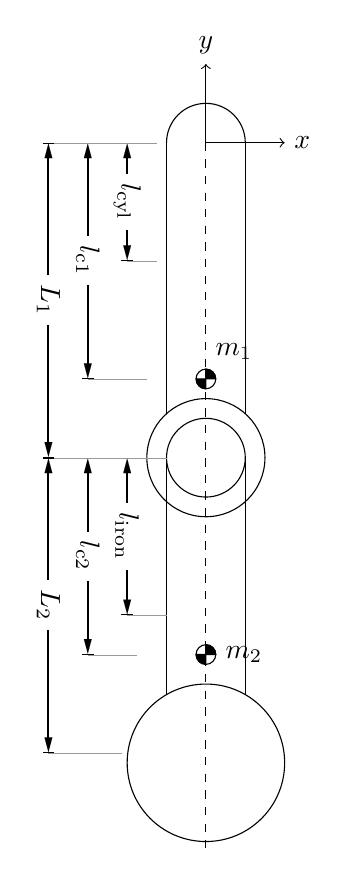
\begin{tikzpicture}[scale=0.5]

\begin{scope}
\clip [rotate=0] (-2,0) rectangle (2,2);
\draw (0,0) circle [radius=1cm];
\end{scope}

\coordinate (O) at (0,0) ;
% Second cirle middle point
\coordinate (A) at (3.5,-6.06217); 
\coordinate (B) at (3.5+6.06217,-6.06217-3.5);
\coordinate (L1) at (0,-6);
\coordinate (L2) at (0,-14);

 
	% Lenght of pendulums are 7cm

	% Axis for underactuated Pendulum
	\draw[->] (0,0) -- (2,0) node[anchor=west] {$x$};
	\draw[->] (0,0) -- (0,2) node[anchor=south] {$y$};
	\draw[dashed] (0,0) -- (0,-2);
	
	%%%%%%%%%%%%%%%%%%%%%%%%%%%%%%%%%%%%%%%%%%%%%%%%%%%%%%%%%%%%%%%%%%%%%%%%%%%%%%

	%%%%%%%%%%%%%%%%%%%%%%%%%%%%%%%%%%%%%%%%%%%%%%%%%%%%%%%%%%%%%%%%%%%%%%%%%%%%%%
	
	%%%%%%%%%%%%%%%%%%%%%%%%%%%%%%%%%%%%%%%%%%%%%%%%%%%%%%%%%%%%%%%%%%%%%%%%%%%%%%
				%% Middle line for underactuated pendulum %%
	\draw[dashed] (O) -- ([yshift=-4cm]L2);
	%%%%%%%%%%%%%%%%%%%%%%%%%%%%%%%%%%%%%%%%%%%%%%%%%%%%%%%%%%%%%%%%%%%%%%%%%%%%%%
	
		
	%%%%%%%%%%%%%%%%%%%%%%%%%%%%%%%%%%%%%%%%%%%%%%%%%%%%%%%%%%%%%%%%%%%%%%%%%%%%%%
					%% Dimensions of underactuated Pendulum %%
	\dimline[line style = {line width=0.7},extension start length=-0.25, extension end length=-0.25]{(-2,0)}{(-2,-3)}{$l_{\text{cyl}}$}
	
	\dimline[line style = {line width=0.7},extension start length=-0.25, extension end length=-0.25]{(-3,0)}{(-3,-6)}{$l_{\text{c1}}$}
	
	\dimline[line style = {line width=0.7},extension start length=-0.25, extension end length=-0.25]{(-4,0)}{(-4,-8)}{$L_{1}$}
	
	%%%%%%%%%%%%%%%%%%%%%%%%%%%%%%%%%%%%%%%%%%%%%%%%%%%%%%%%%%%%%%%%%%%%%%%%%%%%%%

	%Long lines for underactuated pendulum
	\draw[] (-1,0) -- ([xshift=-1cm,yshift=-0.9cm]L1);
	\draw[] (1,0) -- 	([xshift=1cm,yshift=-0.9cm]L1);	
	
	
	
	%%%%%%%%%%%%%%%%%%%%%%%%%%%%%%%%%%%%%%%%%%%%%%%%%%%%%%%%%%%%%%%%%%%%%%%%%%%%%%
					%% Middle circle for both pendulums %%
	\begin{scope}
		%\clip [rotate=00] (0.866+3.5,0.5-6.06217+2) rectangle (-0.866+3.5-2,-0.5-6.06217);
	%4\clip (A) circle [radius=1.02];
	\draw ([yshift=-2cm]L1) circle [radius=1.5cm];
	\draw ([yshift=-2cm]L1) circle [radius=1cm];
	\end{scope}
	
	%\draw [rotate=00] (0.866+3.5,0.5-6.06217+2) rectangle (-0.866+3.5-2,-0.5-6.06217);
	
	%%%%%%%%%%%%%%%%%%%%%%%%%%%%%%%%%%%%%%%%%%%%%%%%%%%%%%%%%%%%%%%%%%%%%%%%%%%%%%
	% Axis for lower Pendulum
	%\draw[->,thick] (3.5,-6.06217) -- (6.5,-6.06217) node[anchor=west] {$x_{2}$};
	%\draw[->,thick] (3.5,-6.06217) -- (3.5,-3.06217) node[anchor=south] {$y_{2}$};
	%\draw[dashed] (3.5,-6.06217) -- (3.5,-8.56217);
	
	% Long lines for actuated pendulum
	%\draw ([xshift=-1cm,yshift=-2cm]L1) rectangle ([xshift=1cm,yshift=2cm]L1);
	\begin{scope}
	\clip ([xshift=-1.5cm,yshift=-2cm]L1) rectangle ([xshift=1.5cm,]L2);
	
	\draw[] ([xshift=-1cm,yshift=-1.5cm]L1) --([xshift=-1cm]L2);
	\draw[]([xshift=1cm,yshift=-1.5cm]L1) --([xshift=1cm,]L2);
	\end{scope}
	
	
	%%%%%%%%%%%%%%%%%%%%%%%%%%%%%%%%%%%%%%%%%%%%%%%%%%%%%%%%%%%%%%%%%%%%%%%%%%%%
	
	%%%%%%%%%%%%%%%%%%%%%%%%%%%%%%%%%%%%%%%%%%%%%%%%%%%%%%%%%%%%%%%%%%%%%%%%%%%%%%
	
	%%%%%%%%%%%%%%%%%%%%%%%%%%%%%%%%%%%%%%%%%%%%%%%%%%%%%%%%%%%%%%%%%%%%%%%%%%%%%%
						%% Dimensions of actuated Pendulum %%
	\dimline[line style = {line width=0.7},extension start length=-0.25, extension end length=-0.25]{(-2,-8)}{(-2,-12)}{$l_{\text{iron}}$}
	
	\dimline[line style = {line width=0.7},extension start length=-0.25, extension end length=-0.25]{(-3,-8)}{(-3,-13)}{$l_{\text{c2}}$}
	
	\dimline[line style = {line width=0.7},extension start length=-0.25, extension end length=-0.25]{(-4,-8)}{(-4,-15.5)}{$L_{2}$}
	
	%%%%%%%%%%%%%%%%%%%%%%%%%%%%%%%%%%%%%%%%%%%%%%%%%%%%%%%%%%%%%%%%%%%%%%%%%%%%%%

	
	%%%%%%%%%%%%%%%%%%%%%%%%%%%%%%%%%%%%%%%%%%%%%%%%%%%%%%%%%%%%%%%%%%%%%%%%%%%%%%
							%% Circle at the bottom %%
	\draw ([yshift=-1.75cm]L2) circle [radius=2cm];
	%%%%%%%%%%%%%%%%%%%%%%%%%%%%%%%%%%%%%%%%%%%%%%%%%%%%%%%%%%%%%%%%%%%%%%%%%%%%%%

	
	%%%%%%%%%%%%%%%%%%%%%%%%%%%%%%%%%%%%%%%%%%%%%%%%%%%%%%%%%%%%%%%%%%%%%%%%%%%%%%


	%%%%%%%%%%%%%%%%%%%%%%%%%%%%%%%%%%%%%%%%%%%%%%%%%%%%%%%%%%%%%%%%%%%%%%%%%%%%%%
				%% Centroid symbol for underactuade pendulum %%
	\draw (0,-6) circle [radius=0.25cm];
	\draw (0,-6-0.25) -- (0,-6+0.25)  node[above right]{$m_{1}$};`
	\draw (0,-6+0.25) -- (0,-6-0.25);
	\filldraw[fill=black,draw=black] (0,-6) -- (0.25,-6)
		arc[start angle = 0, end angle = 90, radius = 0.25] -- cycle;
		
	\filldraw[fill=black,draw=black] (0,-6) -- (-0.25,-6)
	arc[start angle = 180, end angle = 270, radius = 0.25] -- cycle ;
	%%%%%%%%%%%%%%%%%%%%%%%%%%%%%%%%%%%%%%%%%%%%%%%%%%%%%%%%%%%%%%%%%%%%%%%%%%%%%%
	
	%%%%%%%%%%%%%%%%%%%%%%%%%%%%%%%%%%%%%%%%%%%%%%%%%%%%%%%%%%%%%%%%%%%%%%%%%%%%%%
				%% Centroid symbol for actuaded pendulum %%
	\draw (0,-13) circle [radius=0.25cm];
	\draw (-0.25,-13) -- (0.25,-13)  node[right]{$m_{2}$};
	\draw (0,-13+0.25) -- (0,-13-0.25);
	\filldraw[fill=black,draw=black] (0,-13) -- (0.25,-13)
	arc[start angle = 0, end angle = 90, radius = 0.25] -- cycle;
	
	\filldraw[fill=black,draw=black] (0,-13) -- (-0.25,-13)
	arc[start angle = 180, end angle = 270, radius = 0.25] -- cycle ;
	%%%%%%%%%%%%%%%%%%%%%%%%%%%%%%%%%%%%%%%%%%%%%%%%%%%%%%%%%%%%%%%%%%%%%%%%%%%%%%

	
\end{tikzpicture}
\end{document}
	\caption{Simplified Drawing of Physical Model}
	\label{fig:model_drawing}
\end{figure}

Figure \ref{fig:model_drawing} shows a functional drawing of the physical model to visually aid the reader in understanding how the inertia of the system is determine. In equation (\ref{eq:condense1}) and (\ref{eq:condense2}) the $I_{a}$ and $I_{b}$ represents the inertia of the non-actuating and actuated pendulum about the axis coming out of the page passing through the center of mass respectively.\\

The physical model contains many parts that contribute to the inertia of the each pendulum due to representing a different physical form. How the inertia values shown in Table \ref{table:system_param} were determined will be shown below.\\

The actuated pendulum consist out of a aluminium square rod connected to the shaft and the motor mounting. The inertia of a square rod through it's center of mass is: $$ I_{cyl} = \frac{1}{12}m_{cyl}[w^2+L^2_{1}]$$

The motor, gearbox and the motor mount was viewed as a point mass. It's inertia around the center of mass of the non-actuated pendulum is: $$I_{pointmass_1} = m_{pointmass_1}\cdot[L_{1}-l_{c1}]^2 $$

The total inertia of the of the non-actuated pendulum is then: $$ I_{a} =I_{pointmass_1} +  I_{cyl} + m_{cyl}\cdot[l_{c2}-l_{cyl}]^2 $$

The actuated pendulum contains similar parts as the non-actuated pendulum. A pointmass at the bottom and an iron rod connected to the motor shaft and the pointmass. Determining the inertia is thus exactly the same as the non-actuated pendulum.

The physical system parameters used in the preceding text is shown in the Table \ref{table:model_param}


\begin{table}[]
	\centering
	\begin{tabular}{|c|c|c|c|}
		\hline
		Non-Actuated Pendulum& Value & Actuated Pendulum & Value \\
		\hline
		\hline
		$m_{\text{cyl}}$ & \SI{5}{} & $m_{\text{iron}}$ &\\
		\hline
		$w_{\text{cyl}}$ & \SI{3.3}{}& $w_{\text{iron}}$& \\
		\hline
		$m_{\text{pointmass1}}$ & \SI{12}{}& $m_{\text{pointmass2}}$& \\
		\hline
		$l_{\text{cyl}}$ & \SI{12}{}& $l_{\text{iron}}$& \\
		\hline
		$L_{\text{c1}}$ & \SI{12}{} & $L_{\text{c2}}$&\\
		\hline
		$L_{1}$ & \SI{12}{}& $L_{2}$& \\
		\hline
	\end{tabular}
	\caption{Physical Model Paramaters}
	\label{table:model_param}
\end{table}


\subsection{Motor}
The chosen motor used during experiments was the \textit{Faulhaber DC 3257 012 CR} micromotor. It was used in combination with the \textit{Faulhaber Planetary Gearhead 32/3} Series. The gearbox is a 2 stage reduction gearbox with a overall rounded reduction ratio of 14:1. The motor is capable of providing a stall torque of \SI{539}{mNm} which is a converted output torque from the gearbox of \SI{7.646}{Nm}.\\

The motor terminal connection is connected directly to the PCB of the electronic design being routed through the slipring. The motor assembly contains a encoder for position measurements and it's signal and power connection is also routed through the slipring and connected to the PCB.
\subsection{Assembly}



\section{Electronic Hardware}
%WHAT you are going to present in this chapter/section
%WHY you are presenting it, and
%HOW you are going to present it
The electronic hardware was a crucial component for the successful implementation of the robotic gymnast. The electronic design provided the means to determine the system characteristic and verification of the simulated model. It will be presented by discussing the various components implemented to achieve the results in this report.

\subsection{System Description}

% Show block diagram of the system and explain the functioning og the system
\begin{figure}[h]
	\centering
	\input{"./figs/Electronic_System/ElectronicSystemOverview.tikz"}
	\caption{Electronic System Overview}
	\label{fig:electronicSystemOverview}
\end{figure}



Figure \ref{fig:electronicSystemOverview} provides a system overview and how the different parts functions together. The micro-controller receives the different signals that has been correctly conditioned from supporting circuitry to interpret the dynamics of the system. From the observed condition it is able to output the correct signals to instruct the next command.\\

The digital logic circuit that consist of logic level converters acquires the signal from the micro-controller and performs signal conditioning to interface with the motor driver and determines the correct direction to rotate the motor. \\

The motor driver controls the DC brushed motor based of the digital signals and provides a proportional feedback current that is delivered to unity-gain amplifier.\\

The motor contains a encoder that indicates the direction and position of the rotor through digital signals that is sent through a digital logic filter to retrieve only critical information from the encoder signals. \\

The physical model contains a potentiometer that measures the non-actuated pendulums angle and is sent to the buffer.\\

The microcontroller will use the UART interface as it's data acquisition protocol to send the necessary information to the computer. \\

The micro-controller is programmed using the Serial Wire Debug (SWD) protocol to transfer the binaries from the computer.\\

Power is provided using a external 12V power-supply, which will power the motor, but also using a regulator to down convert/step to a 5V and 3.3V to power the microcontoller and the other peripherals.


\subsection{Microcontroller}
The microcontroller chosen is the STM32F030Mxx. The selection was done according the ease of setting up, memory size, physical dimensions and the peripherals it provided.\\

The STM32F030MXX is based of the ARM M0 architecture which is ARM's entry level micro-controller. It requires little support to have a up and running microcontroller requiring only the SWD protocol to program and a few by-pass capacitors.\\

It was difficult to determine the memory size specification for the project. This uncertainty ensured that the largest memory size the ARM M0 architecture could provide was selected.\\

The Electrical and Electronic Department's Printed Circuit Board (PCB) manufacturing machine can only provide a  minimum track width \SI{0.3}{mm}. This resulted in choosing a microcontroller whose footprint would meet the requirement.\\

Based on the conceptual design, the chosen microcontroller required to contain 2 ADC's, minimum of 5 GPIO's and 1 serial communication peripheral.

\subsubsection{Programming / Debug Interface}
The \textit{Atollic TrueSTUDIO for ARM 8.0.0} Integrated Development Environment (IDE) is used for writing the source code which converts the source code to the Executable and Linkable Format (.elf) file. These .elf files is then written using the Serial Wire Debug (SWD) protocol to the $\mu$C. Debugging of the source code occur using the same IDE which allows the programmer to inspect variables, timers and logic.

\subsubsection{PC UART Interface }

The purpose of the UART to serial communication is for data acquisition of the system response and for debugging purposes. The data being sent follows a structure to ensure the reliability of the data. Figure (ref) shows the format of the data being sent.

The data being sent across the UART to serial circuit is retrieved by a computer executing a Python script, listening for any activity on the computer's driver ports and writing the data into a comma-separated value (csv) file that can later be use to analyse the data.


The UART to serial circuit has been tested by doing a loopback test and using a digital logic analyser to verify the data being sent. The loopback test consist of connecting the Tx and Rx lines together and forcefully echo what has been sent to the circuit to be sent back. Figure (ref) in Appendix XXX shows the digital signals sent and received and confirms the working of the UART to Serial circuit. 

\subsection{Voltage Regulation}

The various components required different supply voltages in the electronic design. The diffenrent supply voltage is tabulated in table \ref{table:supplyVoltage}.

\begin{table}[]
	\centering
	\begin{tabular}{|c|c|}
		\hline
		Component & Supply Voltage [\SI{}{V}] \\
		\hline
		\hline
		Digital Logic Components & \SI{5}{} \\
		\hline
		$\mu$Controller & \SI{3.3}{} \\
		\hline
		Motor Driver & \SI{12}{} \\
		\hline
	\end{tabular}
	\caption{Suppy Voltage's for the different components}
	\label{table:supplyVoltage}
\end{table}


The table indicates 3 different supply voltages that will be required: \SI{3.3}{V}, \SI{5}{V} and \SI{12}{V}. This was achieved by using a \SI{5}{V} and \SI{3.3}{V} linear voltage regulators and the \SI{12}{V} is supply by a external source.

The schematic for each voltage regulator is shown in Appendix XX, where each voltage regulator circuit includes a Light Emitting Diode (LED) to ensure the minimum load is met for each regulator. The LED also acts as a visual debugging method.

\subsection{Potentiometer Sensor}
\subsubsection{Working Principle}
\begin{figure}[h]
	\centering
	\input{"figs/potentiometer/potentiometer.tikz"}
	\caption{Simplified Model of a Potentiometer}
	\label{fig:potentiometer}
\end{figure}
The rotary position potentiometer consist out of a wiper that is attached to a rotating shaft. This wiper moves across a internal resistor as the shaft rotates and changes the effective resistance across the output terminal. It provides thus a proportional voltage to it's position as seen in Figure \ref{fig:potentiometer} that indicates the position.

\subsubsection{Interface}
\begin{figure}[h]
	\centering
	\input{"./figs/unitygain/unitygain.tikz"}
	\caption{Unity Gain Amplifier Circuit}
	\label{fig:unitygain}
\end{figure}
The signal produced by the rotary potentiometer varies from 4.95V and 50mV from 360\textdegree \space to 0\textdegree \space respectively. This signal is sent through a simple voltage divider circuit to reduce the signal to 3V and 15mV to be within the sampling limits of the micro-controller. The scaled voltage is sent through a unity gain rail-to-rail amplifier, where the mirrored output signal is fed into the ADC. The type of ADC used in the STM32F030XX is a successive approximation register (SAR) and contains an internal capacitors that suffers from the effect of being depleted if the sampling frequency is to high \citep{stm32_ADC:2017}. Using an operational amplifier reduces the risk of depleting this internal capacitor because of the low output resistance. The schematic of the circuit is shown in Appendix XXX.\\

\subsection{Magnetic Encoder}
\subsubsection{Working Principle}
A rotating gear containing ferrous metal teeth is attach to the rotating shaft. The rotating metal teeth rotates near a hall-effect sensor which creates a change in the magnetic flux inside the hall-sensor. This change in magnetic flux is sensed by the hallsensor which produces a digital signal \citep{hallsensor}.
\subsubsection{Digital Interface} 

\begin{figure}[h]
	\centering
	\input{"figs/JK_XOR_gates/jk_xor_nor.tikz"}
	\caption{Digital Logic Circuit containing JK-Flipflops, XOR- and NOR Gates}
	\label{fig:jk_xor}
\end{figure}

\begin{figure}[h]
	\centering
	\documentclass{article}
\usepackage{tikz-timing}[]
\usepackage{tikz}
\usetikzlibrary{shapes,arrows}
\usepackage{amsmath,bm,times}
\newcommand{\mx}[1]{\mathbf{\bm{#1}}} % Matrix command
\newcommand{\vc}[1]{\mathbf{\bm{#1}}} % Vector command
\pagestyle{empty}
\def\degr{${}^\circ$}



\begin{document}


\def\degr{${}^\circ$}
\begin{tikztimingtable}[]
  PHASE A	       & H   12{2C} G\\
  PHASE B  	       & [C] 12{2C} L \\
  A $\oplus$ B	   & L H L H L H L H L H L H L H L H L H L H L H L H \\
  A$\cdot$A        & C 12{2C}  \\
  Q		       & L 12L 12H \\
  %Final Pulse Set          & 3L 16H N(B5) 6L \\
  %Final Pulse $\overline{\mbox{Reset}}$ & 6L N(B4) 16H 3L \\
  %Final Pulse              & 3L N(B1) 19H N(B8) 3L \\
\extracode
  \tablerules
  %\begin{pgfonlayer}{background}
   % \foreach \n in {1,...,1}
    %  \draw [help lines] (A\n) -- (B\n);
  %\end{pgfonlayer}
\end{tikztimingtable}
%
\end{document}
	\caption{Waveform of the JK-Flipflop,XOR, and NOR Gate Circuit}
	\label{fig:jk_xor_waveform}
\end{figure}

The encoder contains a sold state hallsensor which provides 2 channels with a 90\textdegree \space phase difference between the channels. \citep{faulhaberencoder}. These 2 signals under go a hardware filter that produces 2 signals that indicate the direction of the motor and the incremental position.\\

The hardware filter consist out of XOR, NOR and JK-Flipflop gates shown in Figure \ref{fig:jk_xor} and the schematic in Appendix XXX. The XOR gate produces the incremental change of position of the motor which is than read by the microcontroller using interrupts on rising and falling edges. The encoder provides 16 lines per revolution, equal to a combined 32 rising- \& falling edges per line. The encoder provides 2 lines increasing the resolution to 64. The motor is connected to a gearbox with a reduction stage of 14:1. The encoder will thus rotate 14 times per shaft revolution, increasing the resolution to 896 edges per revolution.\\

 The NOR and JK-Flipflop combination produces the direction of the motor by determining whether phase A leads or lags phase B by 90\textdegree. This leading or lagging is indicate by a logical 1 or 0 which is read by the microntroller.\\
 
 The hardware filter was implemented to reduce the processing time of the micro-controller on the original signals and the waveforms are seen in Figure \ref{fig:jk_xor_waveform}.



\subsection{Motor Driver}
\begin{figure}[h]
	\centering
	\input{"./figs/feedback_current/feedback_current.tikz"}
	\caption{Simplified Circuit of Motor Feedback}
	\label{fig:feedback_current}
\end{figure}


The motor IC chosen is the MC33887. It was selected to based on providing the motor up to 6A of current, while withstanding the high current transients due to the fast switching of a inductive load \citep{motorIC}. The motor driver IC provides the motor with 12V DC which is externally provided by a DC power supply. The schematic of the motor driver is shown in Appendix XXX.

The motor driver IC is connected directly to the motor and responsible for directional and rotational control of the brushed DC motor. The motor driver contains 2 half H-bridges that forms a full H-bridge which are Pulse-Width-Modulated (PWM) to control the speed of the motor and originates from the micro-controller. The selected frequency is 10kHz and is recommended by the manufacturers \cite{motorIC}. As discussed previously, the signals' logic level is first converted and than sent through the AND digital filter before the motor driver receives it.\\

The MC33887 provides a proportional current of $\frac{1}{375}$ of the current flowing through the high-side of the full H-bridge \citep{motorIC}. This current is sent through a resistor of \SI{150}{\Omega} to provide a voltage signal to represent the current. Due to the motor being controlled using PWM, the current is a periodic impulse signal. This problem is overcome by adding a parallel capacitor to the resistor to create a ripple voltage. This ripple voltage is sent through a unity-gain amplifier as seen in Figure \ref{fig:unitygain} before it is sampled by the microcontroller. The $R_{\text{input}}$ resistance is the input resistance that the operational amplifier sees and will be the voltage divider circuit resistance in parallel. This closes the feedback loop to implement torque control by the control system.\\


\subsubsection{Logic Level Converters}
\begin{figure}[h]
	\centering
	\input{"./figs/Logic_Level_Converter/LogicLevelConverterAndInverter.tikz"}
	\caption{Logic Level Converter \& Inverter Circuit}
	\label{fig:interterCirc}
\end{figure}


The microcontroller is required to interface with the motor driver and represent a logical high and low as a \SI{3.3}{V} and \SI{0}{V} respectively. The motor driver IC's logical high threshold is \SI{3.5}{V}. It is thus required to use a logic level converter to allow reliable communication between the two devices.\\

The logic level converter used is shown in Figure \ref{fig:interterCirc} and uses the BSS128 transistor. The circuit shown also acts as a inverter where a logic low, \SI{0}{V} by the microcontroller will be converted to a \SI{5}{V} and a logic high, \SI{3.3}{V} will be converted to \SI{0}{V}. This side effect is overcome by inverting the desired responses in software.


\subsubsection{AND Digitial Circuit}
\begin{figure}[h]
	\centering
	


%\usetikzlibrary{circuits.logic.US} % TiKZ Library for US Logic Circuits.
%\usetikzlibrary{calc,arrows}
\begin{tikzpicture}[every path/.style={},>=triangle 45,circuit logic US, every circuit symbol/.style={}]
	% Logic Gates
	\node[and gate,inputs={nn}, point right] (and1) at (2,-1)    {};
	\node[and gate,inputs={nn}, point right] (and2) at (2,-2)    {};
	\node[not gate, point right] (not1) at (0,-0.5) {};
	
	
	\draw (not1.output)[thick] -| (1,-0.9) -- (and1.input 1);
	
	%Outputs
	\draw (and1.output) [thick]-- (3,-1) node[ocirc,label={right:IN 1} ](in1) {};
	\draw (and2.output) [thick]-- (3,-2) node[ocirc,label={right:IN 2} ](in2) {};
\end{tikzpicture}

	\caption{AND digital logic with inverter}
	\label{fig:andCircuit}
\end{figure}

\begin{figure}[h]
	\centering
	\input{"./figs/and_waveform/and_waveform.tikz"}
	\caption{AND Digital Logic Circuit Waveforms}
	\label{fig:andCircuit_waveform}
\end{figure}

The AND digital gates in combination with a inverter shown in Figure \ref{fig:andCircuit} is responsible for providing the motor IC's with the PWM signal on the correct input of the motor IC.\\ 

The AND circuit receives 2 signals from the microcontroller  after it has been converted to the correct logic level: the PWM signal and a logic level signal indicating the desired direction. Based on the directional signal the AND circuit will switch the PWM signal between the 2 inputs of the motor IC's while holding the other low as seen in Figure \ref{fig:andCircuit_waveform}.\\

This hardware directional control was done in order to reduce the processing time the microcontroller is required to do to switch the generated PWM signal between the 2 inputs of the motor IC.

\subsection{Verification Tests}

\subsubsection{Angle Sensor Measurements}

\subsubsection{Optical Encoder Measurements}

\subsubsection{ PWM Duty Cycle to Motor Current}

\begin{figure}[h]
	\centering
	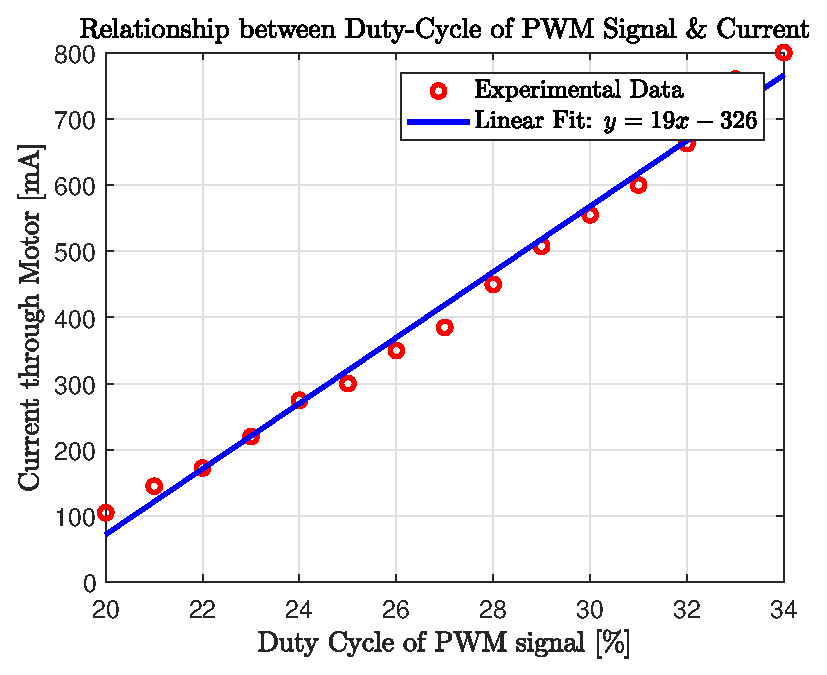
\includegraphics[scale=1]{./figs/dutycycle_vs_current.eps}
	\caption{Relationship between Duty-Cycle of PWM Signal and Current through Motor}
	\label{fig:dutycycle_vs_current}
\end{figure}

The input to the system is the torque delivered by the motor and the magnitude and direction is determined by the control laws. The model describing the system in equation (\ref{eq:condense2}) assumes the torque delivered to the system is instantaneously available. This is inaccurate due to the model describing the DC motor is a second-order differential equation containing it's own time-constant. This model was not incorporated due adding another control loop would add more delays to the control systems. To overcome this, the torque provided by the motor would be mapped to the duty-cycle the motor receives.\\

Experiments were done to determine the relationship between the duty-cycle of the PWM signal and the torque delivered by the motor. These experiments are done by incrementing the duty-cycle of the PWM signal that the motor receives when the shaft is kept fix against a hard-stop. The mean value of the output voltage from the circuit shown in \ref{fig:feedback_current} was measured on the oscilloscope and mapped backwards to determine the torque using equation (\ref{eq:duty2current}) with the constant shown in Table \ref{table:duty2current_constants0.}
\begin{equation} \label{eq:duty2current}
\tau = \frac{V}{R}\cdot GR \cdot FR \cdot \alpha_{t}
\end{equation}

\begin{table}[]
	\centering
	\begin{tabular}{|c|c|c|}
		\hline
		Constant & Description & Value \\
		\hline
		\hline
		GR &  Gear Ratio & 14 \\
		\hline
		FR & Feedback Current Ratio & 375 \\
		\hline
		$\alpha_{t}$ & Torque Constant & $19.1\times 10^{-3}$ \\
		\hline
		R & Resistance & 150 \\
		\hline
	\end{tabular}
	\caption{Values of Constants used in Equation (\ref{eq:duty2current})}
	\label{table:duty2current_constants}
\end{table}

 Figure \ref{fig:dutycycle_vs_current} shows the measured data with a line of best fit. It is clear that there exist a linear relationship between the duty-cycle of the PWM signal and the torque provided. This equation of best fit will thus be used to output the correct torque determined by the control system.

